\documentclass[final,hyperref={pdfpagelabels=false}]{beamer}
\mode<presentation>{\usetheme{Lankton}}
\boldmath
\usepackage{times}
\usepackage{ragged2e} 
\usepackage{caption}
\usepackage{graphicx}
\usepackage{subcaption}
\usepackage{amsmath,amsthm, amssymb, latexsym}
\usepackage[english]{babel}
\usepackage[latin1]{inputenc}
\usepackage{graphicx}
\graphicspath{{figures/}}
\setbeamertemplate{caption}[numbered]
\usepackage[orientation=landscape,size=a1,scale=1]{beamerposter}

\title{SyntenyFinder: A Synteny Blocks Generation and Genome Comparison Tool}
\author{Ilya Minkin\textsuperscript{1}, Nikolay Vyahhi\textsuperscript{1}, and Son Pham\textsuperscript{2}}
\institute{\textsuperscript{1} St. Petersburg Academic University, St. Petersburg, Russia \\ \textsuperscript{2} University of California, San Diego, USA}

\begin{document}
\begin{frame}{}

\begin{columns}[t]

\begin{column}{0.32\linewidth}

\begin{block}{Introduction} \justifying
Recent advances in sequencing and genome assembling technologies are resulting in many finished genomes.
The comparison of these genomes has been emerging as a powerful tool for genome interpretations and has led to many important scientific discoveries.
The genome comparison tasks often require genomes to be  decomposed to a collection of synteny blocks -- long regions of conserved DNA.

[Here we insert a colorful picture about synteny blocks]

Currently existing tools can reconstruct synteny blocks from genomes represented as sequences of enumerated local alignments, or \textit{anchors}.
We propose \textit{SyntenyFinder} -- a tool for finding synteny blocks in genomes represented as nucleotide sequences. Our approach is based on de Bruijn graph
and can be applied to closely related genomes.
\end{block}

\begin{block}{De Bruijn graphs} \justifying
\(K\)-dimensional de Bruijn graph \(G(k)\) is a graph which vertex set consists of all possible \(k\)-length strings over the alphabet \(\lbrace A, C, G, T \rbrace\). 
For each \((k + 1)\) - substring \(w\) in the given string \(S\) we add to \(G(k)\) an edge that connects \(k\)-prefix of \(w\) with \(k\)-suffix of \(w\) and label the edge with
index of the first character of \(w\).
\begin{figure}
	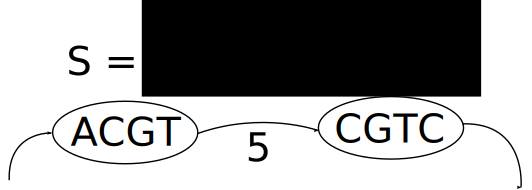
\includegraphics[scale = 0.6]{deBruijnEdge.pdf}
	\small \caption{Forming edge set of a \(4\)-dimensional de Bruijn graph}
\end{figure}
In this graph we allow only paths that have consecutive labels on edges, so each valid path spells a substring from \(S\).
Non-branching paths in the graph \(G(k)\) indicate repeats in the string \(S\), i.e. synteny blocks. But in real genomes
synteny blocks contain variations that disrupt non-branching paths. These variations create so called \textit{bulges} in
the graph. In order to reconstruct synteny blocks we must \textit{simplify} the graph.
\end{block}

\end{column}

\begin{column}{0.32\linewidth}

\begin{block}{SyntenyFinder algorithm} \justifying
Given two numbers \(k\) and \(\delta\) and a set \(S = \lbrace S_{1}, S_{2}, \ldots, S_{n} \rbrace \) of chromosomes 
represented as nucleotide strings, our algorithm works as follows:
\begin{itemize}
\item Concatenate all string in \(S\) into the supergenome \(\hat{S}\)
\item Construct graph \(G_+(k)\) from \(\hat{S}\) and color all it's edges \textit{blue}
\item Construct graph \(G_-(k)\) from reverse-complementary of \(\hat{S}\) and color all it's edges \textit{red}
\item Obtain \(G(k) = G_+(k) \cup G_-(k)\) and change \(\hat{S}\) so that \(G(k)\) doesn't contain bulges with both branches having size \( < \delta \)
\item Output non-branching paths
\end{itemize}
At any moment during simplification there is one-to-one correspondence between the string \(\hat{S}\) and the graph -- any changes in \(\hat{S}\) are immediately reflected in \(G(k)\).
\end{block}

\begin{figure}
\begin{figure}
        \begin{subfigure}[a]{1\textwidth}
		\centering
		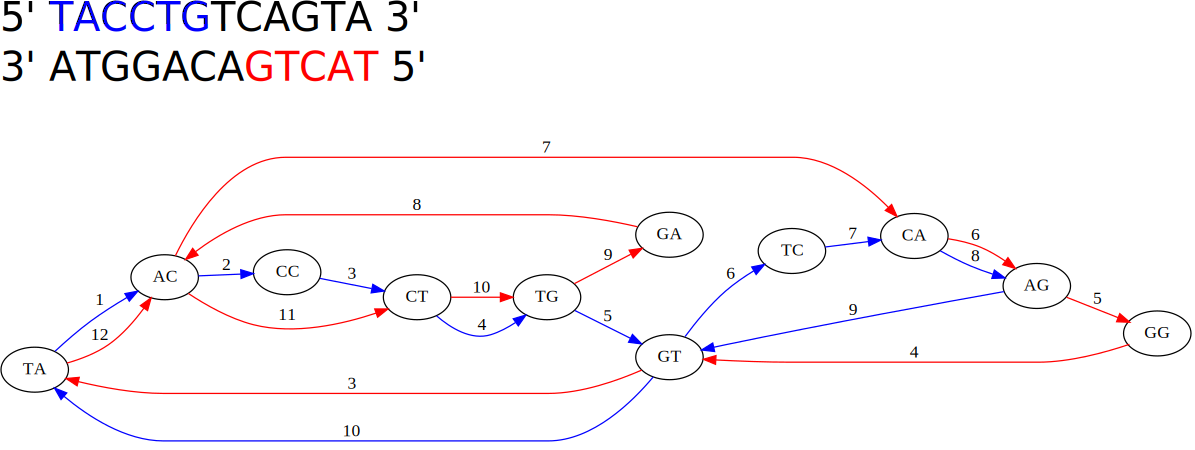
\includegraphics[scale = 0.75]{graph1.pdf}
		\justifying
		\small \caption{De Bruijn graph \(G(k)\) built from \(\hat{S} = "TACCTGTCAGTA"\). Two paths \(("AC", "CC", "CT")\) and \(("AC", "CT"\)) form
		a \textit{bulge} that indicate an indel in the substrings \("ACCT"\) and \("ACT"\). }
		\label{DeBruijnA}
        \end{subfigure}
        \begin{subfigure}[b]{1\textwidth}
		\centering
		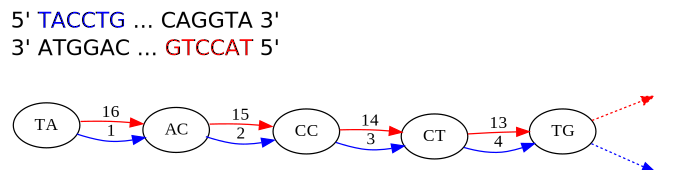
\includegraphics[scale = 0.75]{graph2.pdf}
		\small \caption{The same graph after collapsing the bulge. Now long non-branching path spells synteny block \("TACCTG"\).}
		\label{DeBruijnB}
        \end{subfigure}
	\small \caption{Illustration of \textit{de Bruijn} graphs and simplification process}
\end{figure}

\end{figure}

\end{column}

\begin{column}{0.32\linewidth}

\begin{block}{Results} \justifying
You can make a poster very quickly and easily by cutting and pasting the \LaTeX~codes from the paper!
\end{block}

\begin{block}{Discussion} \justifying
You can make a poster very quickly and easily by cutting and pasting the \LaTeX~codes from the paper!
\end{block}

\begin{block}{References} \justifying
You can make a poster very quickly and easily by cutting and pasting the \LaTeX~codes from the paper!
\end{block}

\begin{block}{Acknowledgments} \justifying
This work was supported by the Government of the Russian Federation (grant 11.G34.31.0018)
and the National Institutes of Health (NIH grant 3P41RR024851-02S1).
\end{block}

\end{column}

\end{columns}

\end{frame}
\end{document}